To better understand the system's intended functionality from a user's perspective, a use case analysis was performed. To this end, a use case diagram was designed, which is an effective tool for visualizing the interactions between external actors and the system, thereby defining its functional scope.

In this system, the primary actor is the \textbf{User}, a general user representing all use cases of the system. Figure~\ref{FIG:USE_CASE} illustrates the main functionalities available to the actors \textbf{User} and \textbf{Guest User}, with the latter being, exclusively, a non-authenticated user. These use cases cover the entire spectrum of user interaction with the platform, from initial account management to the creation of and conversation with recommender agents. The principal use cases are:

\begin{description}
    \item[Manage Account:] Encompasses all functionalities related to user account management, including registration, login, password reset, and viewing the personal \acs{api} access key.
    \item[Manage Recommender Agents:] Includes the complete lifecycle of an agent: creating a new agent from datasets, browsing the Agent Hub, editing agent metadata, retraining and deleting an agent.
    \item[Use Agent Chat:] Represents the core conversational feature, where a user engages in a dialogue with a specific, trained recommender agent to receive recommendations.
    \item[Use Open Chat:] Refers to the general-purpose chat interface where a user can converse freely with an \ac{llm}, with support for advanced features like web search and file uploads.
\end{description}

\begin{figure}[System Use Case Diagram]{FIG:USE_CASE}{System Use Case Diagram.}
    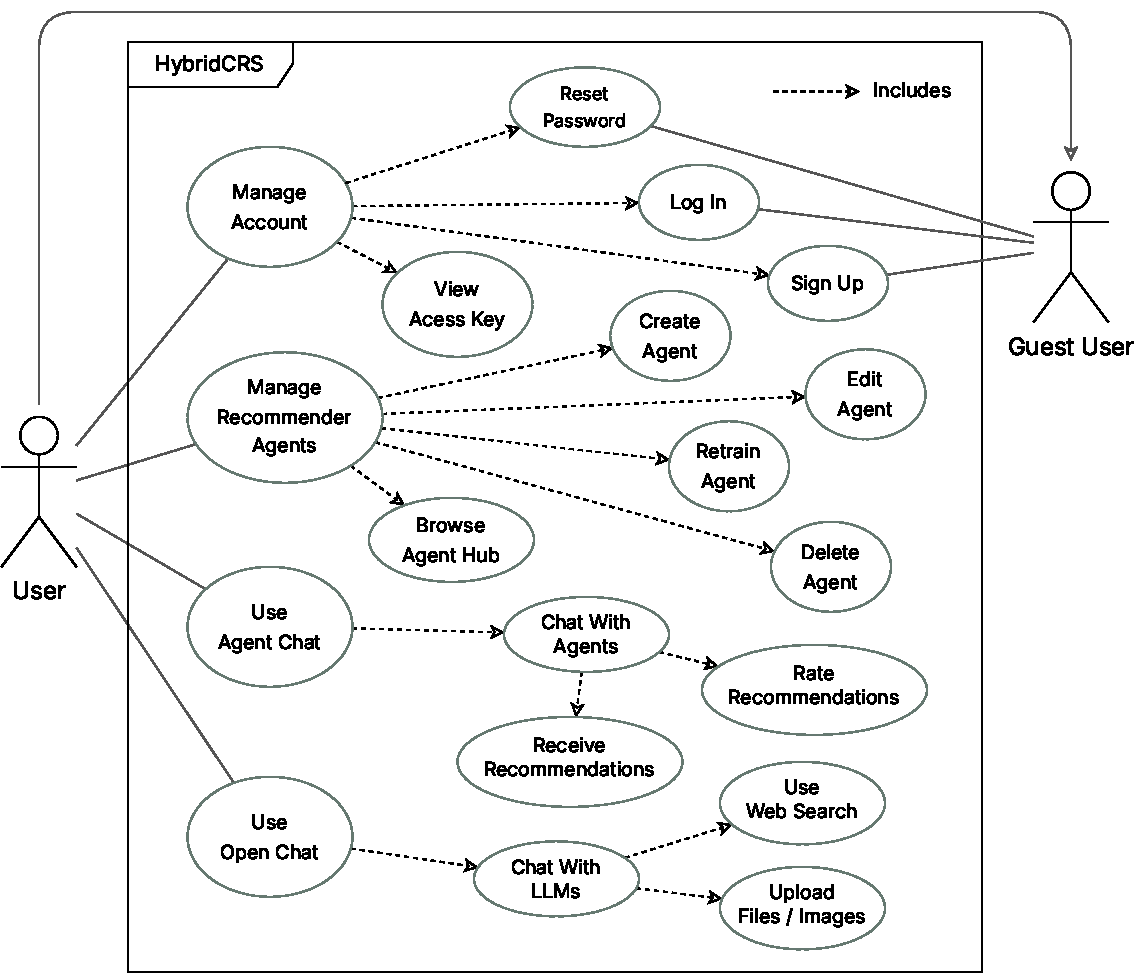
\includegraphics[width=\textwidth]{use_case.pdf}
\end{figure}
